\documentclass[a4paper,UTF8]{article}
\usepackage{ctex}
\usepackage[margin=1.25in]{geometry}
\usepackage{color}
\usepackage{graphicx}
\usepackage{amssymb}
\usepackage{amsmath}
\usepackage{amsthm}
\usepackage{enumerate}
\usepackage{bm}
\usepackage{hyperref}
\usepackage{epsfig}
\usepackage{color}
\usepackage{mdframed}
\usepackage{lipsum}
\usepackage{mathtools}
\usepackage{hyperref}
\usepackage{diagbox}
\usepackage{float}
\usepackage{caption}
\usepackage{algorithm}
\usepackage{algorithmicx}  
\usepackage{algpseudocode}
\usepackage{amsmath} 
\usepackage{graphicx}
\newmdtheoremenv{thm-box}{myThm}
\newmdtheoremenv{prop-box}{Proposition}
\newmdtheoremenv{def-box}{定义}
\usepackage{listings}
\usepackage{xcolor}
\lstset{
	numbers=left, 
	numberstyle= \tiny, 
	keywordstyle= \color{ blue!70},
	commentstyle= \color{red!50!green!50!blue!50}, 
	frame=shadowbox, % 阴影效果
	rulesepcolor= \color{ red!20!green!20!blue!20} ,
	escapeinside=``, % 英文分号中可写入中文
	xleftmargin=2em,xrightmargin=2em, aboveskip=1em,
	framexleftmargin=2em
} 

\usepackage{booktabs}

\setlength{\evensidemargin}{.25in}
\setlength{\textwidth}{6in}
\setlength{\topmargin}{-0.5in}
\setlength{\topmargin}{-0.5in}

% \setlength{\textheight}{9.5in}
%%%%%%%%%%%%%%%%%%此处用于设置页眉页脚%%%%%%%%%%%%%%%%%%
\usepackage{fancyhdr}                                
\usepackage{lastpage}                                           
\usepackage{layout}                                             
\footskip = 10pt 
\pagestyle{fancy}                    % 设置页眉                 
\lhead{研一下学期}                    
\chead{论文阅读笔记}                                                
% \rhead{第\thepage/\pageref{LastPage}页} 
\rhead{Step1}                                                                                               
\cfoot{\thepage}                                                
\renewcommand{\headrulewidth}{1pt}  			%页眉线宽,设为0可以去页眉线
\setlength{\skip\footins}{0.5cm}    			%脚注与正文的距离           
\renewcommand{\footrulewidth}{0pt}  			%页脚线宽,设为0可以去页脚线

\makeatletter 									%设置双线页眉                                        
\def\headrule{{\if@fancyplain\let\headrulewidth\plainheadrulewidth\fi%
\hrule\@height 1.0pt \@width\headwidth\vskip1pt	%上面线为1pt粗  
\hrule\@height 0.5pt\@width\headwidth  			%下面0.5pt粗            
\vskip-2\headrulewidth\vskip-1pt}      			%两条线的距离1pt        
 \vspace{6mm}}     								%双线与下面正文之间的垂直间距              
\makeatother  

%%%%%%%%%%%%%%%%%%%%%%%%%%%%%%%%%%%%%%%%%%%%%%
\numberwithin{equation}{section}
%\usepackage[thmmarks, amsmath, thref]{ntheorem}
\newtheorem{theorem}{Theorem}
\newtheorem*{definition}{Definition}
\newtheorem*{solution}{Solution}
\newtheorem*{prove}{Proof}
\newcommand{\indep}{\rotatebox[origin=c]{90}{$\models$}}

\usepackage{multirow}

%--

%--
\begin{document}
\title{论文阅读笔记\\
Step1}
\author{MF1833063, 史鹏, spwannasing@gmail.com}
\maketitle
\newpage
\section{Chinese Poetry Generation with Planning based Neural Network}
这篇论文主要介绍了一种seq2seq的模型,用于生成古诗,根据输入的文本:一句话或者一篇文章,
生成表达对应含义的古诗。
\begin{enumerate}
	\item 提出了一种“planning-based”诗歌生成框架,这个框架明确的规划每一行的子主题。
	\item 修改了RNN的encoder-decoder框架,使其同时支持对于子主题以及前面已经生成的行进行编码,逐行的生成诗句。 
    \begin{figure}[htbp]
        \centering
        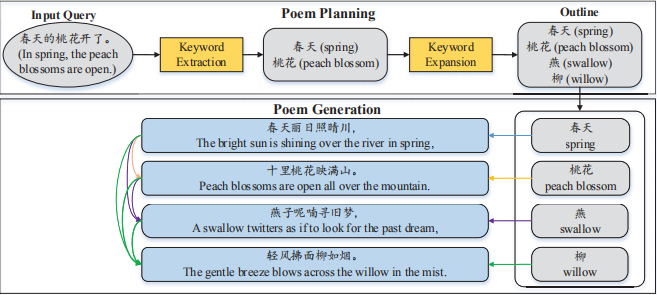
\includegraphics[height=7.5cm,width=15cm]{framework.jpg}
        \caption{整体工作流程}
    \end{figure}
    \item   对于提取用户输入的文本中的关键词使用了TextRank算法。\\
    TextRank算法基于PageRank,用于为文本生成关键字和摘要。\\
    \begin{figure}[H]
        \centering
        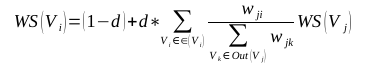
\includegraphics[height=1.3cm,width=6cm]{textrank.png}
        \caption{权重计算公式}
    \end{figure}
    思想:(1)如果一个单词出现在很多单词后面的话,那么说明这个单词比较重要\\
    (2)一个TextRank值很高的单词后面跟着的一个单词,那么这个单词的TextRank值会相应地因此而提高
    \newpage
    \item 扩充关键词,用户输入的文本提取出的关键词的数量可能不足,这篇论文提出了两种方式解决这个问题。\\
        \subitem{[1]} RNNLM-based方法\\
        使用RNN语言模型来根据已有的关键词序列预测下一个关键词,自动对训练数据根据TextRank算法生成每行诗的关键词,用这些关键词序列来训练RNNLM。
        \subitem{[2]} Knowledge-based方法\\
        利用外部的知识,比如wiki百科,抽取出在这些预料中,已有关键词附近的词,同时这些词还要是名词或者形容词,而且这个词在诗歌训练集中出现过。

    \item 诗歌生成\\
    \begin{figure}[H]
        \centering
        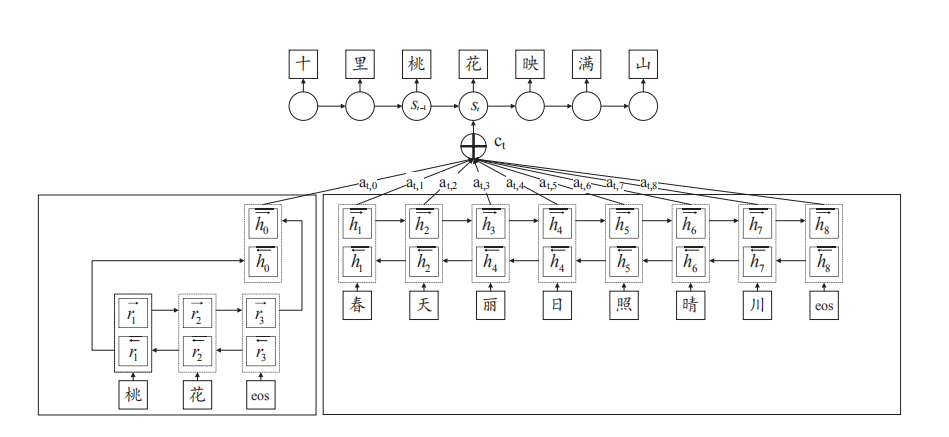
\includegraphics[height=8cm,width=16cm]{model.png}
        \caption{诗歌生成模型}
    \end{figure}
    $$ y_{t}=\mathop{\arg\min}_{y}P(y|s_t,c_t,y_{t-1})$$
    $$ s_t = f(s_{t-1},c_{t-1},y_{t-1})$$
    $$ c_t = \sum_{j=0}^{T_h-1}a_{tj}h_j$$
    $$ a_{tj} = \frac{exp(e_{tj})}{\sum_{t=0}^{T_h-1}exp(e_{tk})}$$
    $$ e_{tj} = v_a^T tanh(W_{a}s_{t-1}+U_{a}h_j)$$

\end{enumerate}

\newpage
\section{MEMORY NETWORKS}
描述了一种新的学习模型,叫做记忆网络,记忆网络推理结合了长期记忆组件和推理组件,学习如何共同使用这些组件。
\begin{enumerate}
    \item RNN等网络结构,因为总是将序列编码到固定长度,所以其记忆能力有限,难以记住一些复杂的信息,甚至是复制自己这种简单的任务都不可以。
    \item 本文的中心思想是将可读写的记忆组件与成功的推理学习策略结合起来。记忆网络由四个组件组成。I、G、O、R    
        \subitem I:input feature map--将输入转化为内部的特征表示。
        \subitem G:generalization--根据输入更新“记忆”内的参数,我们称之为泛化,因为在这个阶段,网络有机会压缩和压缩它的记忆,以供将来使用。
        \subitem O:output feature map--根据输入和当前的记忆,来输出
        \subitem R:response--将上一步的输出转化为文字
    \item 最简单的G的形式是将I(x)存入它记忆的槽(slot)内。$$m_{H(x)}=I(x)$$这里面H(x)的作用是选择一个合适的槽。更复杂的G变体可以根据当前输入x中的新特征,返回并更新先前存储的内存(可能是所有内存)。
    如果内存满了,当H选择替换哪个内存时,它也可以实现一个“遗忘”过程,例如,H可以计算每个内存的效用,选择作用最小的。
    \item 推理的核心是O和R,O通常对于输入x使用寻找"k supporting memories"的方法。
    这里假设k=2,则
    $$ o_{1} = O_{1}(x,m)=\mathop{\arg \max}_{i=1,...,N}s_{O}(x,m_i) $$
    $$ o_{2}=O_{2}(x,m)=\mathop{\arg \max}_{i=1,...,N}s_{O}([x,m_{o1}],m_i)$$
    对于图4中的例子,$m_{o1}$ = “Joe left the milk”,$m_{o2}$ = “Joe travelled to the office”
    然后在$[x, m_{o1}, m_{o2}]$的基础上,对各单词score。选出得分最高的单词。
    \begin{figure}[H]
        \centering
        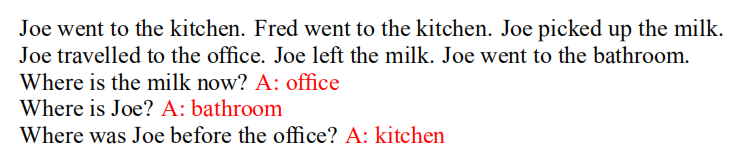
\includegraphics[height=3cm,width=13cm]{example1.png}
        \caption{例子}
    \end{figure}
\end{enumerate} 

\newpage
\section{Teaching Machines to Read and Comprehend}
当前缺少大规模的问答预料,本文的贡献是用一种特殊的方法生成了大规模的有监督阅读理解数据。另外还提出了基于Attention的深度神经网络来进行阅读和回答问题(baseline)。
\begin{enumerate}
    \item 观察到,摘要和句子及其相关文档可以很容易地通过简单的实体检测和算法转换为上下文查询答案。
    \begin{figure}[H]
        \centering
        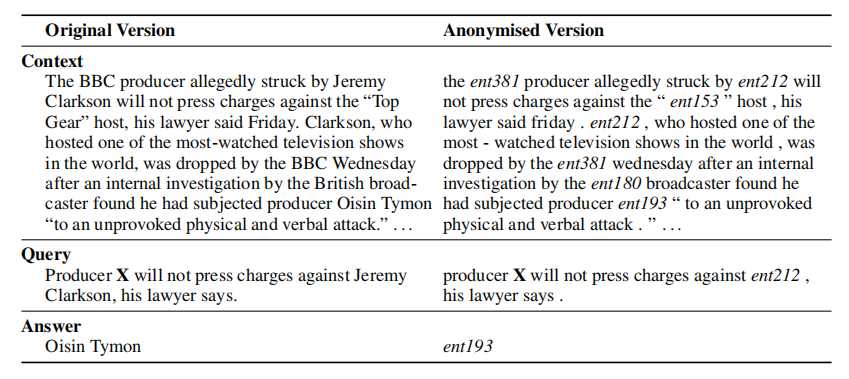
\includegraphics[height=8cm,width=16cm]{corpus.png}
        \caption{示例}
    \end{figure}
    \item 计算某单词作为答案的概率:$p(a|d,q) \propto exp(W(a)g(d,q)$,W(a)是关于a索引的矩阵,g(d,q)返回的是一个关于document和query的向量。
    以下讨论的问题即为获取到g(d,q)的几种方式。
    \item 提出了三种利用神经网络进行计算的方式。
        \subitem{[1]} The Deep LSTM Reader-将query和document用分隔符连接起来,作为一整个sequence送入LSTM,然后把最后一个时间步的每一层连接起来。$$ g^{LSTM}(d,q)=y(|d|,|q|)$$
        \subitem{[2]} The Attentive Reader-对于document中的每一个token都进行相似度计算,得到一个“attention”权重,按权重相加。$$g^{AR}(d,q)=tanh(W_{rg}r+W_{ug}u)$$
        \subitem{[3]} The Impatient Reader-Attentive读者可以专注于上下文文档中最有可能为查询提供答案的段落。我们可以通过对模型进行更深层次的改造,使模型具有更强的可重复性从文档中读取每个查询token。每检索到query中的一个token就将已检索过的query中的tokens 和 document都再看一遍。
    $g^{IR}(d,q)=tanh(W_{rg}r(|q|)+W_{qg}u) $
    \begin{figure}[H]
        \centering
        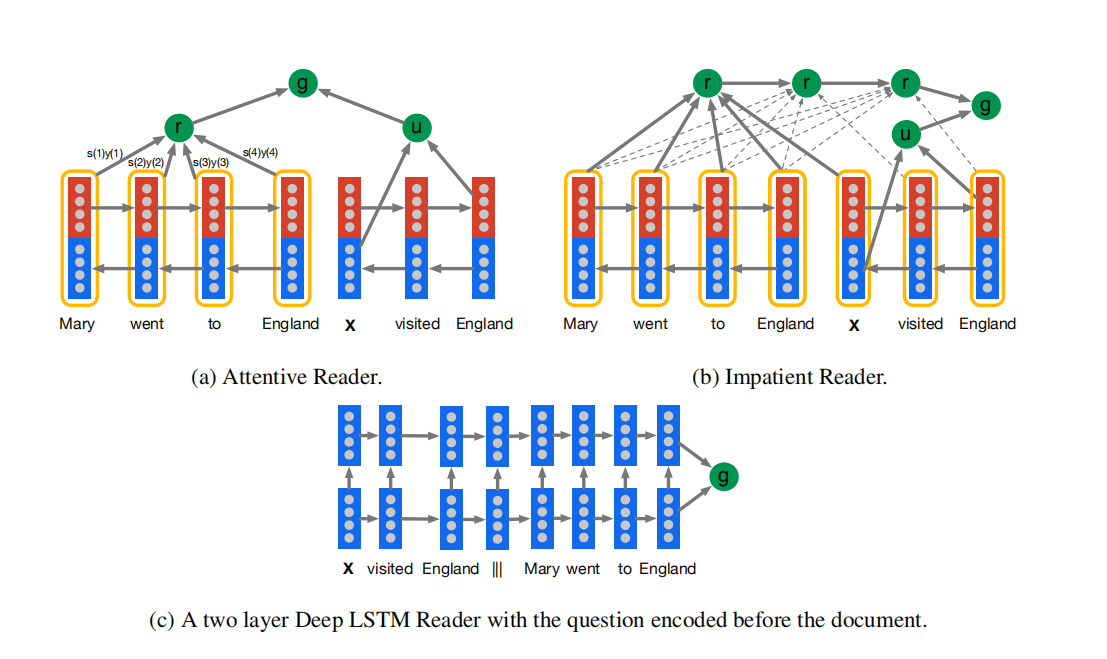
\includegraphics[height=8cm,width=14cm]{attentive.png}
        \caption{三种计算方式}
    \end{figure}
\end{enumerate}

\newpage
\section{Text Understanding with the Attention Sum Reader Network}
提出了一个新的、简单的模型,它使用注意直接从上下文中选择答案,而不是像通常那样使用文档中的混合词表示来计算答案。
\begin{figure}[H]
    \centering
    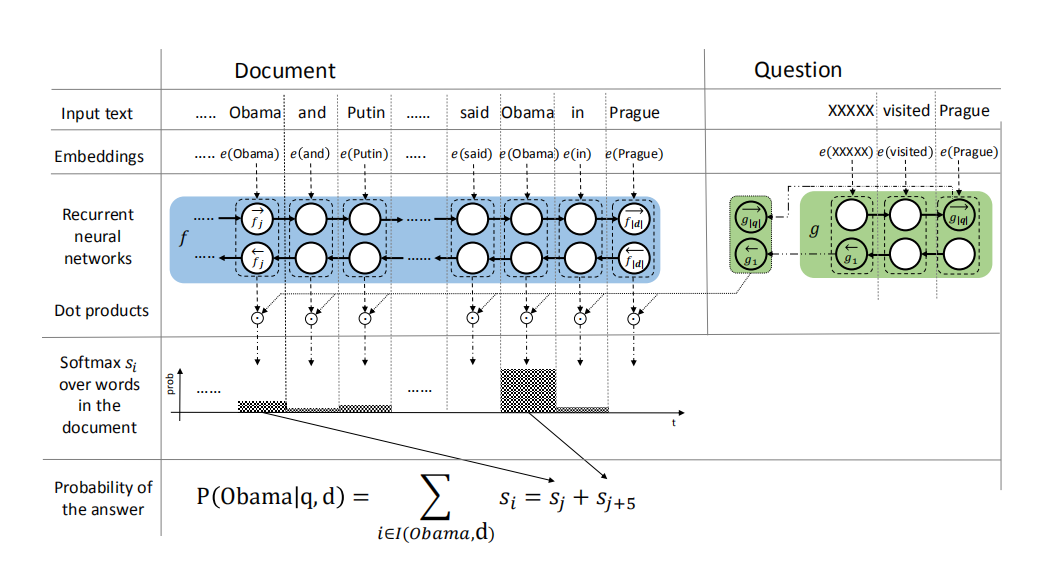
\includegraphics[width=\textwidth]{9-1.png}
\end{figure}
工作流程:\\
(1)计算query的embedding\\
(2)计算document中每个词的contextual embedding\\
(3)点乘,选择最有可能的答案


\newpage
\section{A Thorough Examination of the CNN/Daily Mail Reading Comprehension Task}
主要目标是,弄清楚究竟需要对语言多深的理解才能够完成Reading comprehension的任务。其次提出一个超过目前state-of-art 5\%的模型,并且认为这是这个任务上所能够达到的最高水平。
\begin{enumerate}
    \item Entity-Centric Classifier-为每一个entity设计一个向量$f_{p,q}(e)$,以及学习一个权重矩阵$\theta$使得正确答案的分数比其它答案都要高。
    $$\theta ^{T}f_{p,q}(a)>\theta ^{T}f_{p,q}(e),\forall e \in E \cap\backslash\{a\}$$
    \begin{figure}[H]
        \centering
        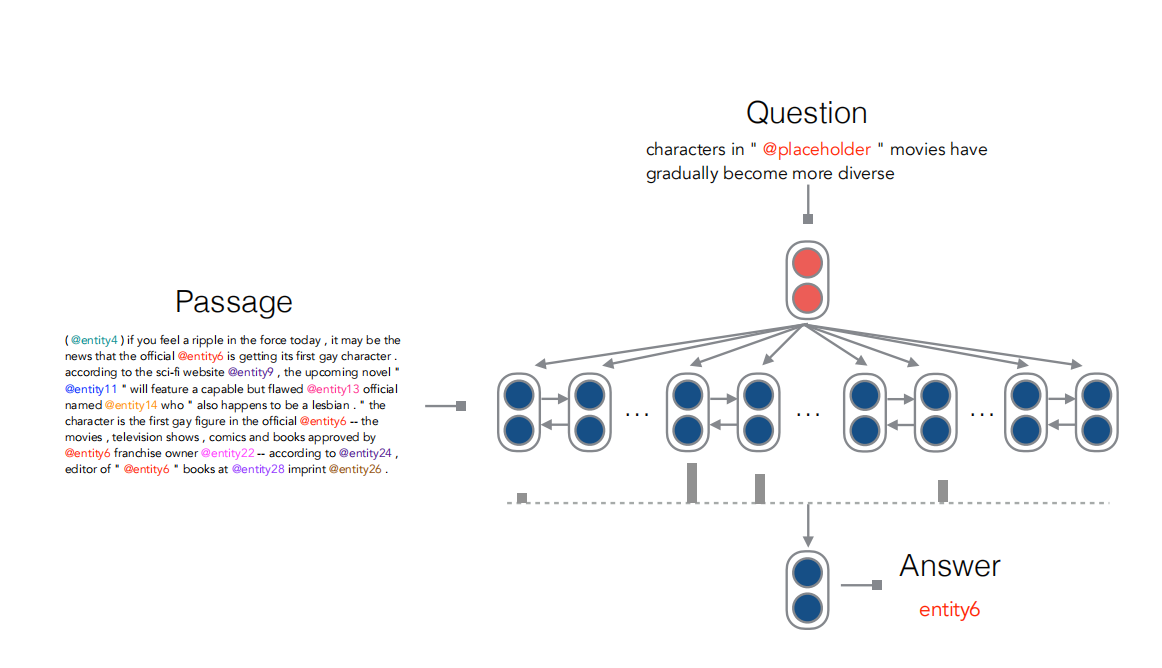
\includegraphics[width=\textwidth]{10-1.png}
        \caption{网络结构}
    \end{figure}
    \item 整体类似Attentive Readder模型,区别就是改进了Attentive Reader里面计算g(d,q)函数的计算方法,将tanh替换为先计算softmax再加权求和。
\end{enumerate}

\newpage
\section{Long Short-Term Memory-Networks for Machine Reading}
本文针对RNN对于处理固定输入的局限性,提出了一种基于LSTM的改进模型。
\begin{figure}[H]
    \centering
    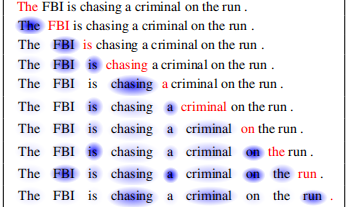
\includegraphics[]{6-2.png}
    \caption{example}
\end{figure}
\begin{enumerate}
    \item 本文所提出的结构的中心思想是使用多个记忆槽(memory slot)来存储输入的表示,而每个槽的read和write操作被建模为Attention机制。Attention不需要监督信息,能够发现输入的token之间的关系。
    \item Long Short-Term Memory (LSTM)$$ \begin{bmatrix}
        i_t\\ 
        f_t\\ 
        o_t\\
        \hat{c_t}
        \end{bmatrix} = \begin{bmatrix}
            \sigma\\ 
            \sigma\\ 
            \sigma\\
            tanh
            \end{bmatrix}W\cdot[h_{t-1},x_t]$$
            $$c_t = f_t \odot c_{t-1}+i_t \odot \hat{c_t}$$
            $$ h_t = o_t \odot tanh(c_t)$$
            \begin{figure}[H]
                \centering
                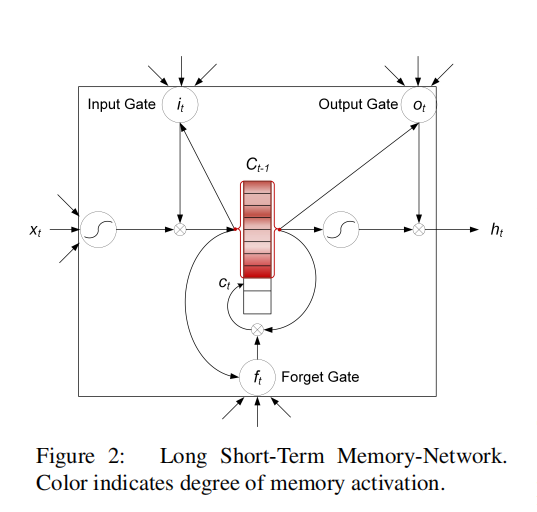
\includegraphics[width=8cm,height=8cm]{6-1.png}
                \caption{网络结构}
            \end{figure}
    \item Long Short-Term Memory-Network(LSTMN)\\将标准LSTM中的memory cell替换为memory network,这样就可以将每一个input的embedding都存入一个不同的memory slot直到达到数量上限。
    而且这样的设计还可以使得能够通过一层neural attention来推理tokens之间的关系。因为在read的时候就是根据目前的token,在所有存储的memories中寻找有用的内容。\\
    对于input gate和forget gate的更新则首先将所有的memories加权相加,剩余的步骤一样。
    \begin{figure}[H]
        \centering
        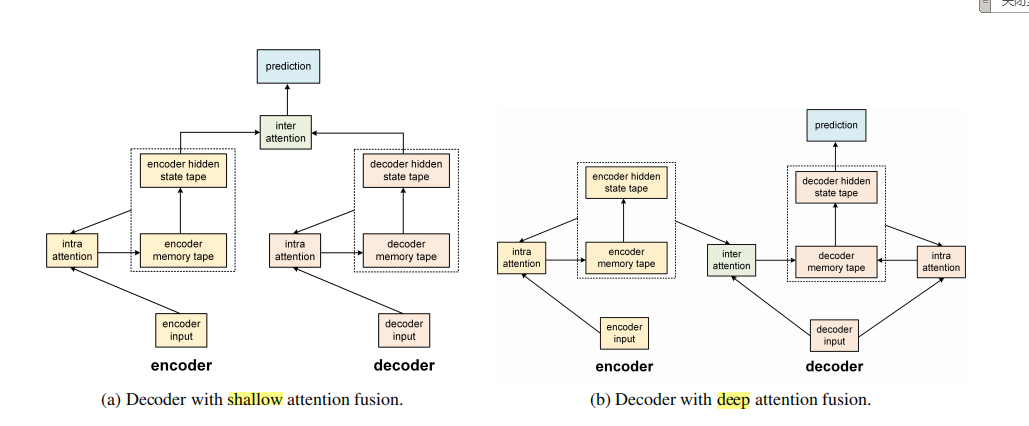
\includegraphics[width=\textwidth]{6-3.png}
        \caption{seq2seq的两种形式}
    \end{figure}

    
\end{enumerate}
\newpage
\section{Key-Value Memory Networks for Directly Reading Documents}
提出了一种全新的键值对记忆神经网络,来改善直接阅读文档的能力。因为它可以在读取memory操作中的寻址(K)和输出(V)两个阶段使用不同的编码。
\begin{enumerate}
    \begin{figure}[H]
        \centering
        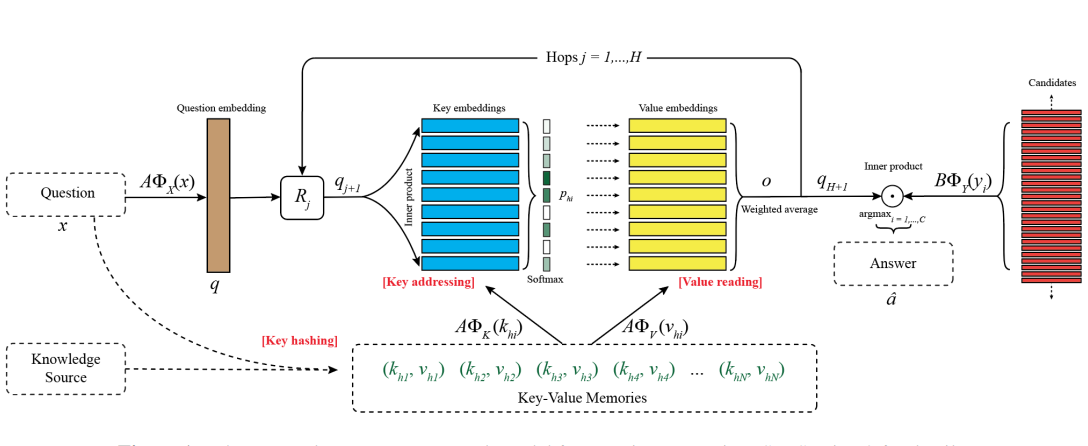
\includegraphics[width=\textwidth]{7-1.png}
        \caption{网络结构}
    \end{figure}
    \item 首先,将事实存储在键值结构化内存中,然后再对它们进行推理,以预测答案。
    \item 存储器的设计使得模型能够学习使用键来寻址与问题相关的存储器,相应的值随后被返回。此结构允许模型为当前任务编码先验知识,并利用键和值之间可能存在的复杂转换。
\end{enumerate}
\newpage
\section{Modeling Human Reading with Neural Attention}

\newpage
\section{LEARNING RECURRENT SPAN REPRESENTATIONS FOR EXTRACTIVE QUESTION ANSWERING}

\newpage
\section{Multi-Perspective Context Matching for Machine Comprehension}

\newpage
\section{Natural Language Comprehension with the EpiReader}

\end{document}